\documentclass[11pt]{article}
\setlength\parindent{0pt}
\usepackage{amsmath}
\usepackage{amsfonts}
\usepackage{graphicx}
\newcommand{\reffig}[1]{[Figure \ref{#1}]}
\title{Music Visualization Algorithm}
\author{Zachary Kieda\\{Advisor: Jesse Stiles}}
\date{\today}
\begin{document}
\maketitle


Our music visualization display is a closed form display that is generated with two different parameters. In this report we will give an overview of what the generated output is and the generating function. We will then discuss how the parameters modify the qualitative features of the generated output. In section three we discuss the mathematics behind the visualization that we see, and finally in the fourth section we discuss methods of controlling these two parameters in the context of music generation. 

\begin{section}{Program Output}
\begin{figure}[h]
\centering
\includegraphics[width=.9\textwidth]{viz-small.png}
\caption{Visualization with $\alpha = .01$, $\lambda = 1$}
\label{fig:vizsmall}
\end{figure}

\begin{figure}[h]
\centering
\includegraphics[width=.9\textwidth]{viz-large.png}
\caption{Visualization with $\alpha = .3$, $\lambda = 1$}
\label{fig:vizlarge}
\end{figure}

The color that we output for each pixel $(x, y)$ we generate a single grayscale color $f(x, y) \in \{k \in \mathbb{N}|0 \le k \le 255\}$. We have example output when zoomed in \reffig{fig:vizsmall}, and output when zoomed out \reffig{fig:vizlarge}. 



\begin{subsection}{Generating Function}
Let $(x, y)$ be pixels on the screen such that the origin $(0, 0)$ is at the center. Let $\lambda, \alpha \in \mathbb{R}$. The grayscale pattern formed is 
\[f(x, y) = \alpha (x^2 + y^2)^\lambda \mod 255 \]
Mathematically, this function is uninteresting. If we can view this with infinite precision and $\lambda = 1$, we would merely get a hypergeometric paraboloid that goes back to zero in bands. The spacing of these bands decrease as $x^2$ and $y^2$ increase. Indeed, we see this occur when $\alpha$ is very small \reffig{fig:vizsmall}. However, we get a more interesting result when $\alpha$ gets large. We start to see the function take on a recursive behavior even though the solution is closed form! As $\alpha$ grows, we see a large variation in behavior -- which is interesting coming from a single function.\\


We note that when $\alpha = 255 + \alpha'$,
\begin{align*}
f(x, y) &= (255 + \alpha') (x^2 + y^2)^\lambda &\mod 255 \\
&\equiv 255(x^2 + y^2)^\lambda + \alpha'(x^2+y^2)^\lambda & \mod 255\\
&\equiv \alpha' (x^2 + y^2)^\lambda & \mod 255
\end{align*}
Mathematically, we have shown that the function recurses back to its original function when $\alpha$ goes past 255. This is actually not true for very large $\alpha$ due to floating point errors, which will produce variation for large $\alpha$, but we'll assume that they're roughly equivalent.\\
\end{subsection}
\begin{subsection}{Visualization at various $\alpha$}
We show a variety of figures where $\alpha \approx 11$, $\alpha \approx 50$, $\alpha \approx 150$, and $\alpha = 254.85$. Note that in the last one this is similar to a smaller value of $\alpha$. \\

Note: Zoom in to see the details of the image -- the details change as you zoom in (and for a good reason, which we'll explain in Section 3).
\begin{center}
\includegraphics[width=.9\textwidth]{viz-11.png}\\
Figure 3: Visualization with $\alpha \approx 11$ and $\lambda = 1$
\label{fig:viz11}
\end{center}
\stepcounter{figure}
\begin{figure}[h]
\centering
\includegraphics[width=.9\textwidth]{viz-50.png}
\caption{Visualization with $\alpha \approx 50$ and $\lambda = 1$}
\label{fig:viz50}
\end{figure}
\begin{figure}[h]
\centering
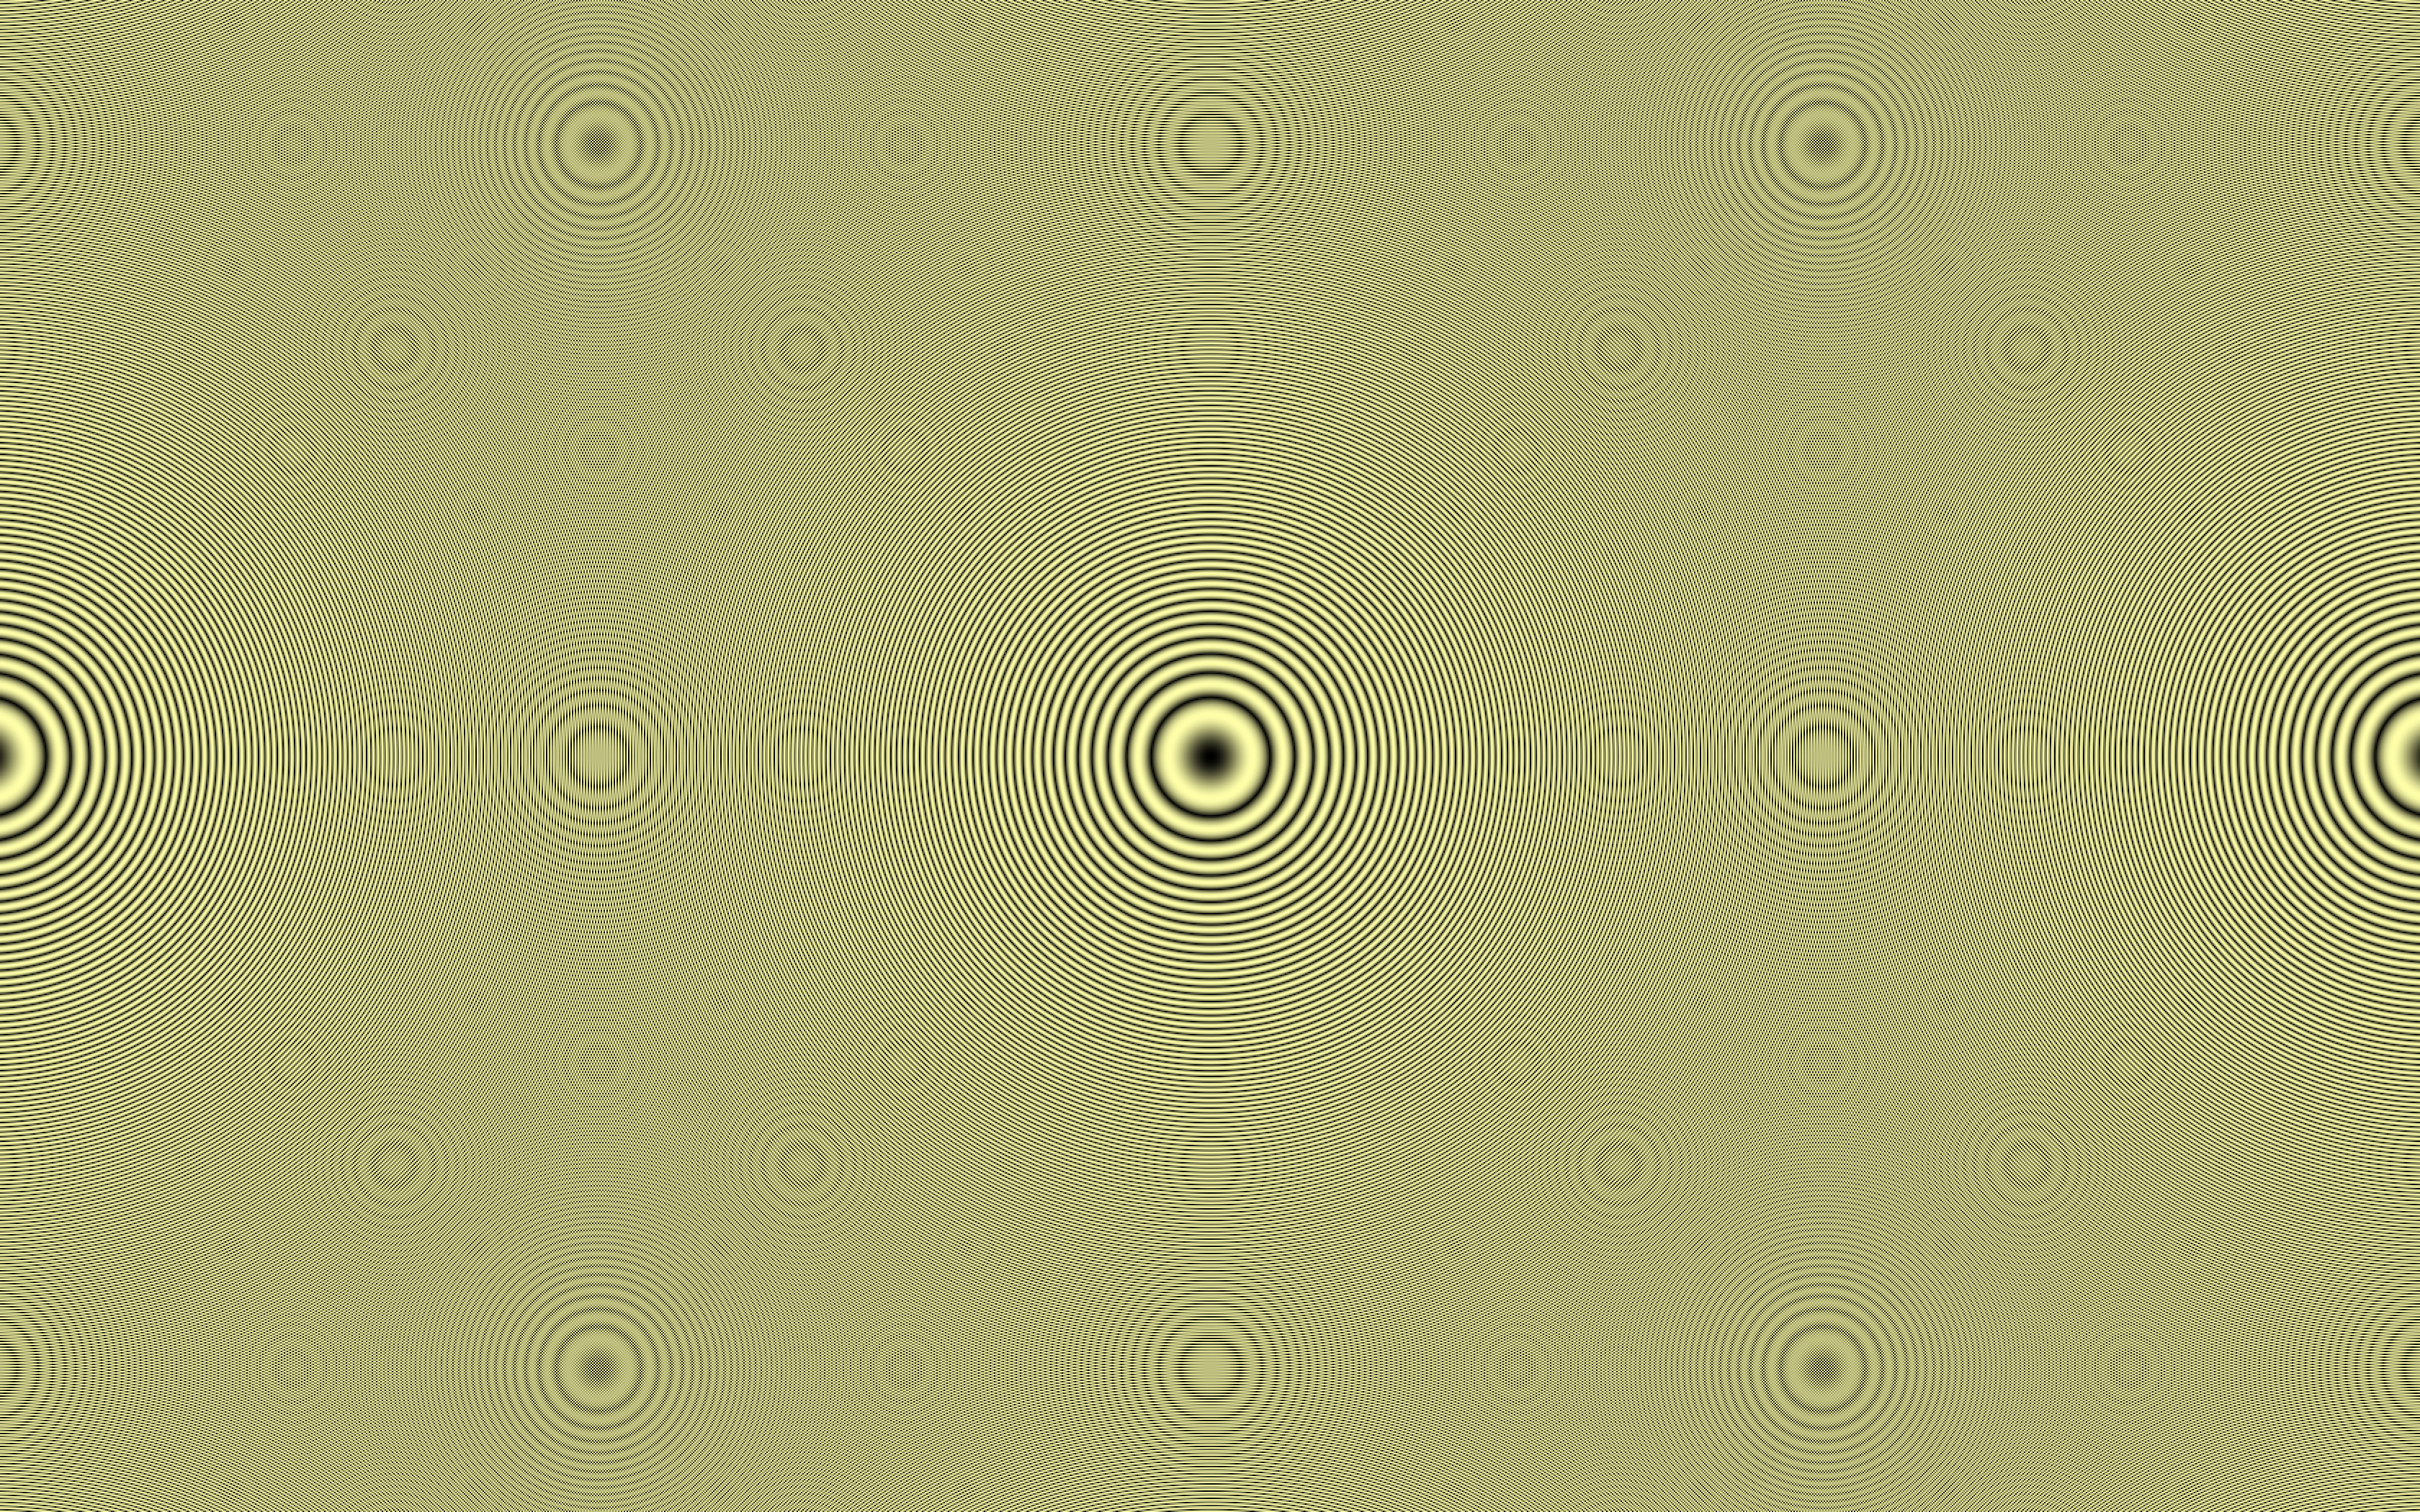
\includegraphics[width=.9\textwidth]{viz-25485.png}
\caption{Visualization with $\alpha = 254.85$ and $\lambda = 1$}
\label{fig:viz25485}
\end{figure}


\end{subsection}
\end{section}
\clearpage
\begin{section}{Additional Qualitative Features and the $\lambda$ Parameter}
The $\lambda$ parameter skews our visualization around the center depending on its value. We define several key intervals
\[\textsf{Look} = \begin{cases}
\textsf{Inverted} & \lambda < 0\\
\textsf{Boring} & \lambda = 0\\
\textsf{Concave/Inverted} & 0 < \lambda < .5\\
\textsf{Linear} & \lambda = .5\\
\textsf{Concave} & .5 < \lambda < 1\\
\textsf{Normal} & \lambda = 1\\
\textsf{Convex} & 1 < \lambda
\end{cases}\]

In our cases when lambda is equal to a particular number, we can easily reason about mathematically. We will not discuss the case \textsf{Normal} here, as we have discussed it above.
\begin{subsection}{Case {\normalfont\textsf{Boring}}, When $\lambda = 0$.}
\begin{figure}[h]
\centering
\includegraphics[width=.9\textwidth]{boring.png}
\caption{Boring. Visualization with $\alpha = .1$ and $\lambda = 0$}
\label{fig:boring}
\end{figure}
We show an example screenshot of when $\lambda = 0$ in \reffig{fig:boring}. 

Note how this scene is rather boring. This is because at this lambda $f(x, y) = \alpha(x^2 + y^2)^0 \mod 255 = \alpha \mod 255$. This is in line with the fact that our visualization is uniform. 
\end{subsection}
\begin{subsection}{Case {\normalfont\textsf{Linear}}, When $\lambda = .5$.}

This is also an uninteresting case, since the visualization is rather uniform through most values of $\alpha$. Mathematically, we have $\alpha(x^2 + y^2)^{.5}$ which is equivalent to the distance from $(0, 0)$ to $(x, y)$. \\
\begin{figure}[h]
\centering
\includegraphics[width=.9\textwidth]{linear-small.png}
\caption{Linear. Visualization with $\alpha = .001$ and $\lambda = .5$}
\label{fig:linearSmall}
\end{figure}
\begin{figure}[h]
\centering
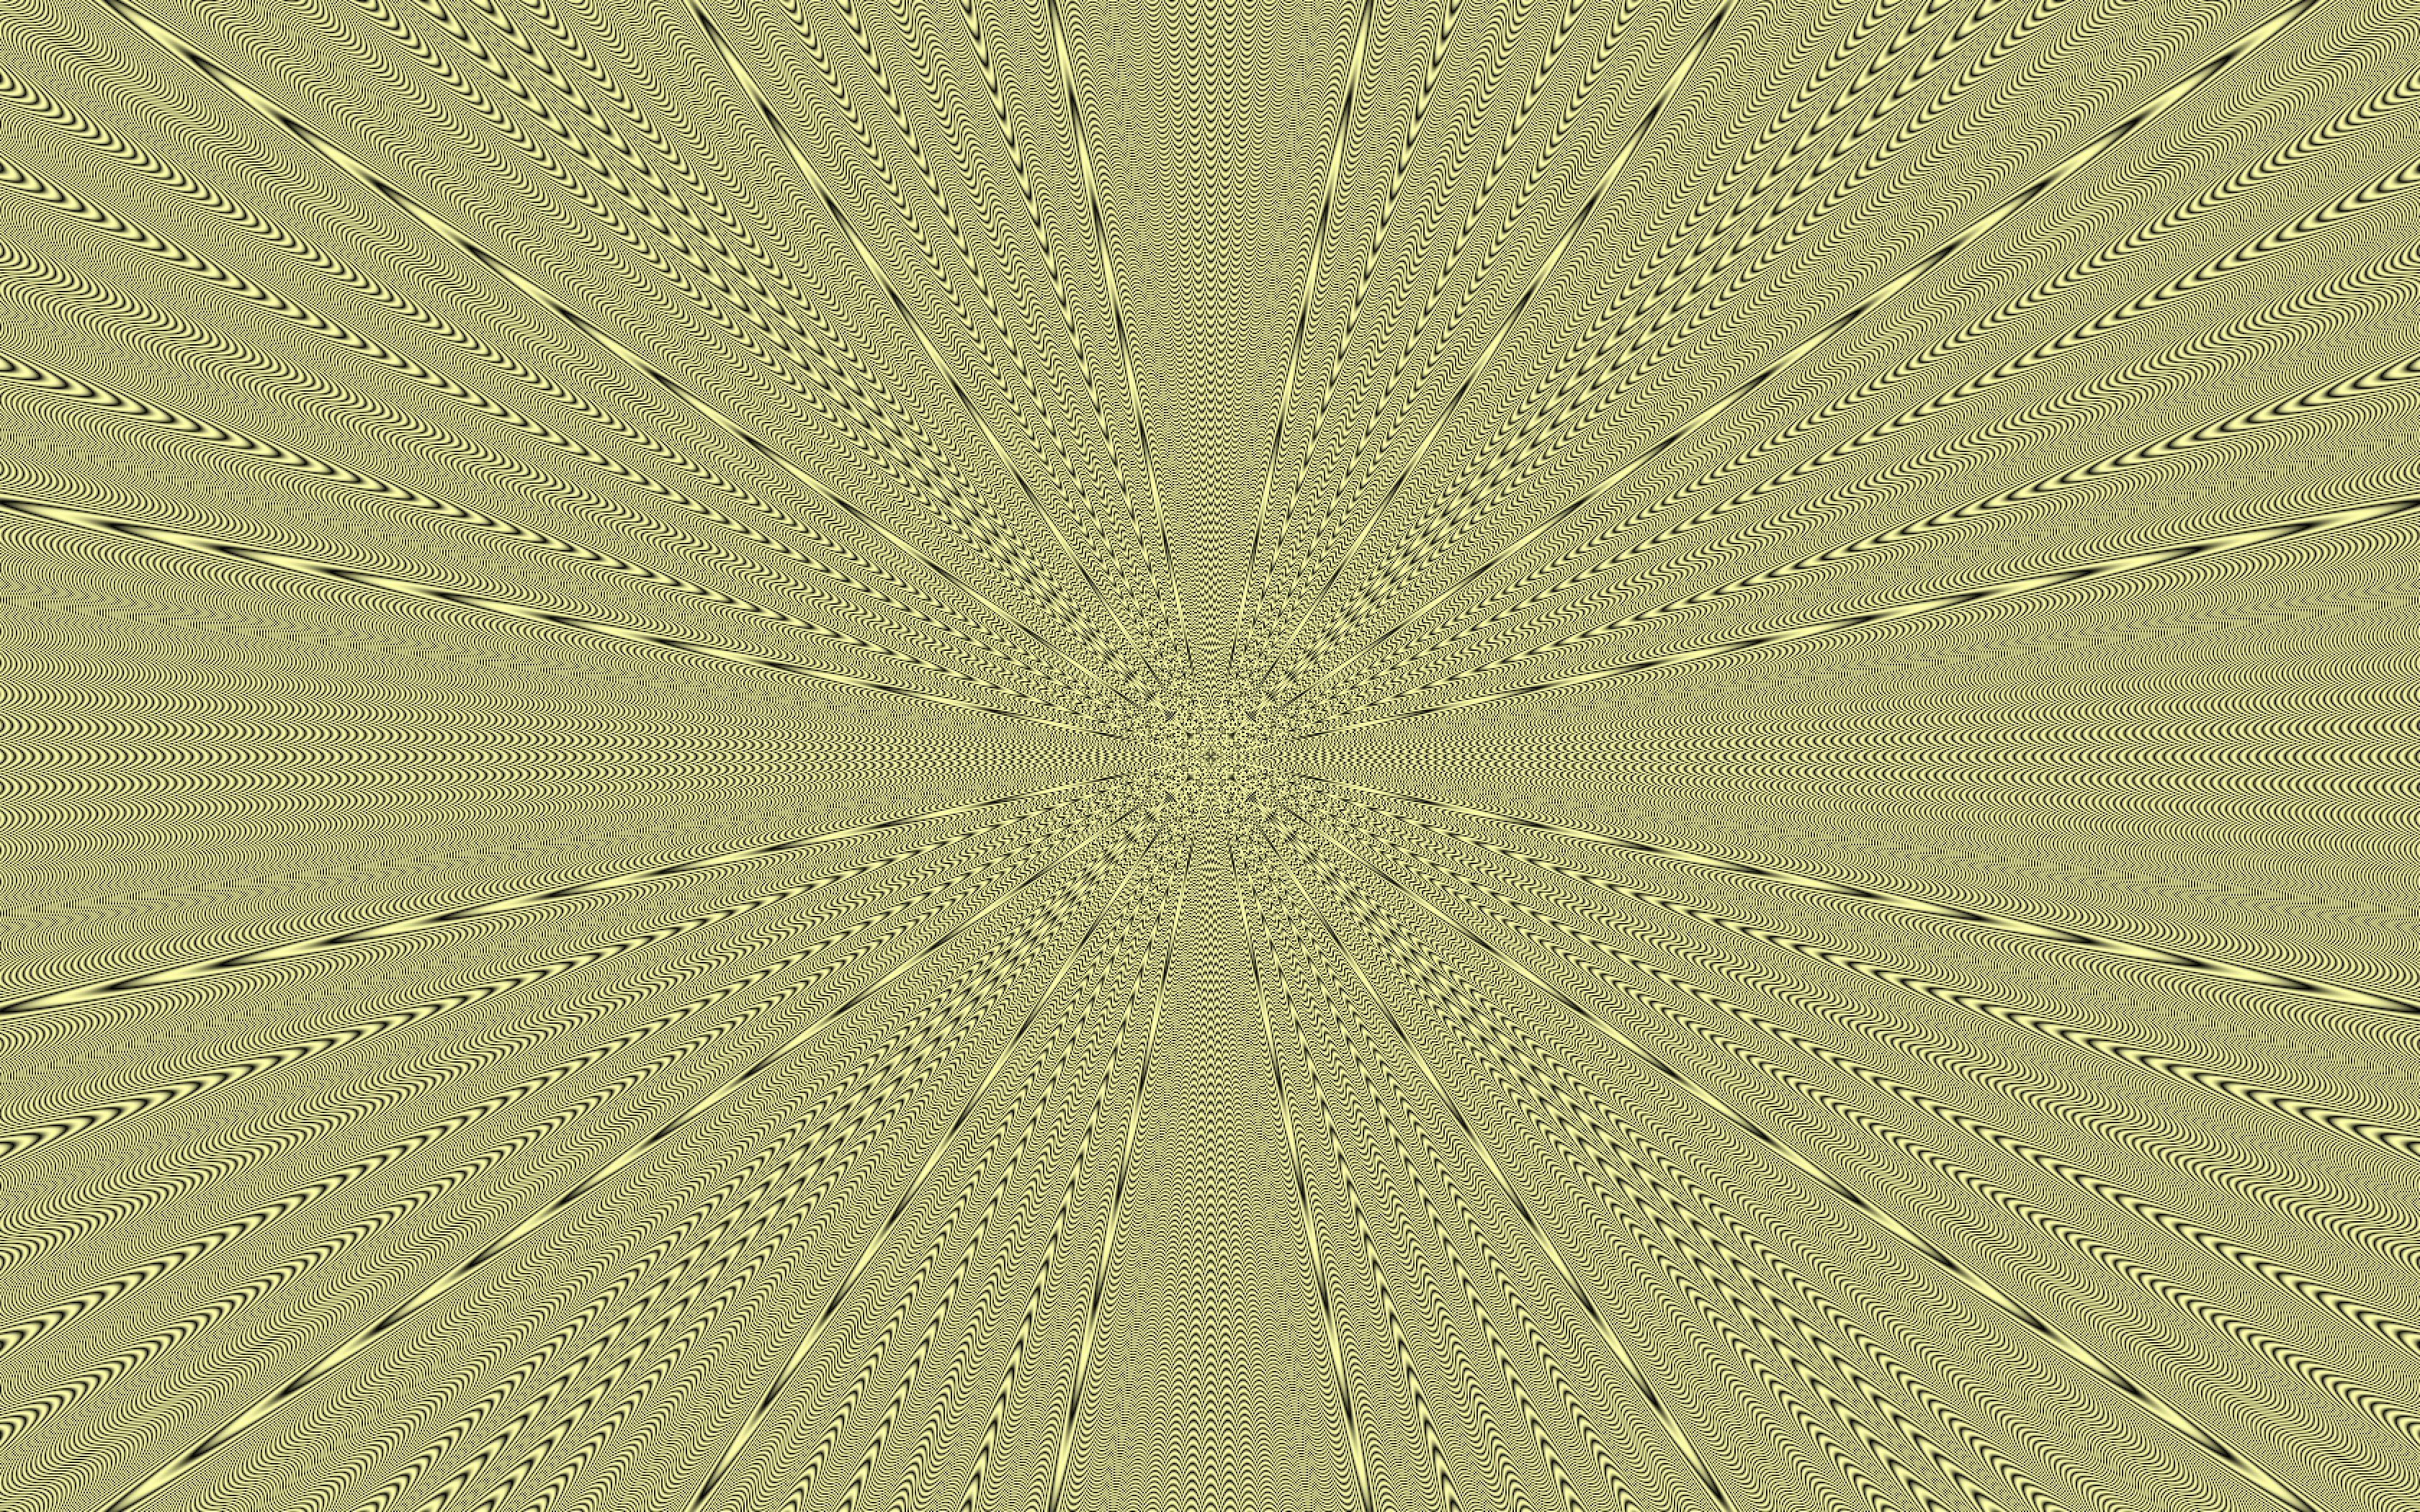
\includegraphics[width=.9\textwidth]{linear-large.png}
\caption{Linear. Visualization with $\alpha = 10$ and $\lambda = .5$}
\label{fig:linearLarge}
\end{figure}
For smaller $\alpha$ we have a series of evenly spaced rings \reffig{fig:linearSmall}, then for large $\alpha$ the image deforms to the pixels on the screen, causing a mildly amusing pattern \reffig{fig:linearLarge}. 
\end{subsection}
\begin{subsection}{Other Cases}
For the inverted cases, as we expect, there's a higher amount of detail as we approach the point $(0, 0)$. Note that the concave case makes our function pulls more to the middle, whereas the convex case pushes the middle outwards. 
\begin{figure}[h]
\centering
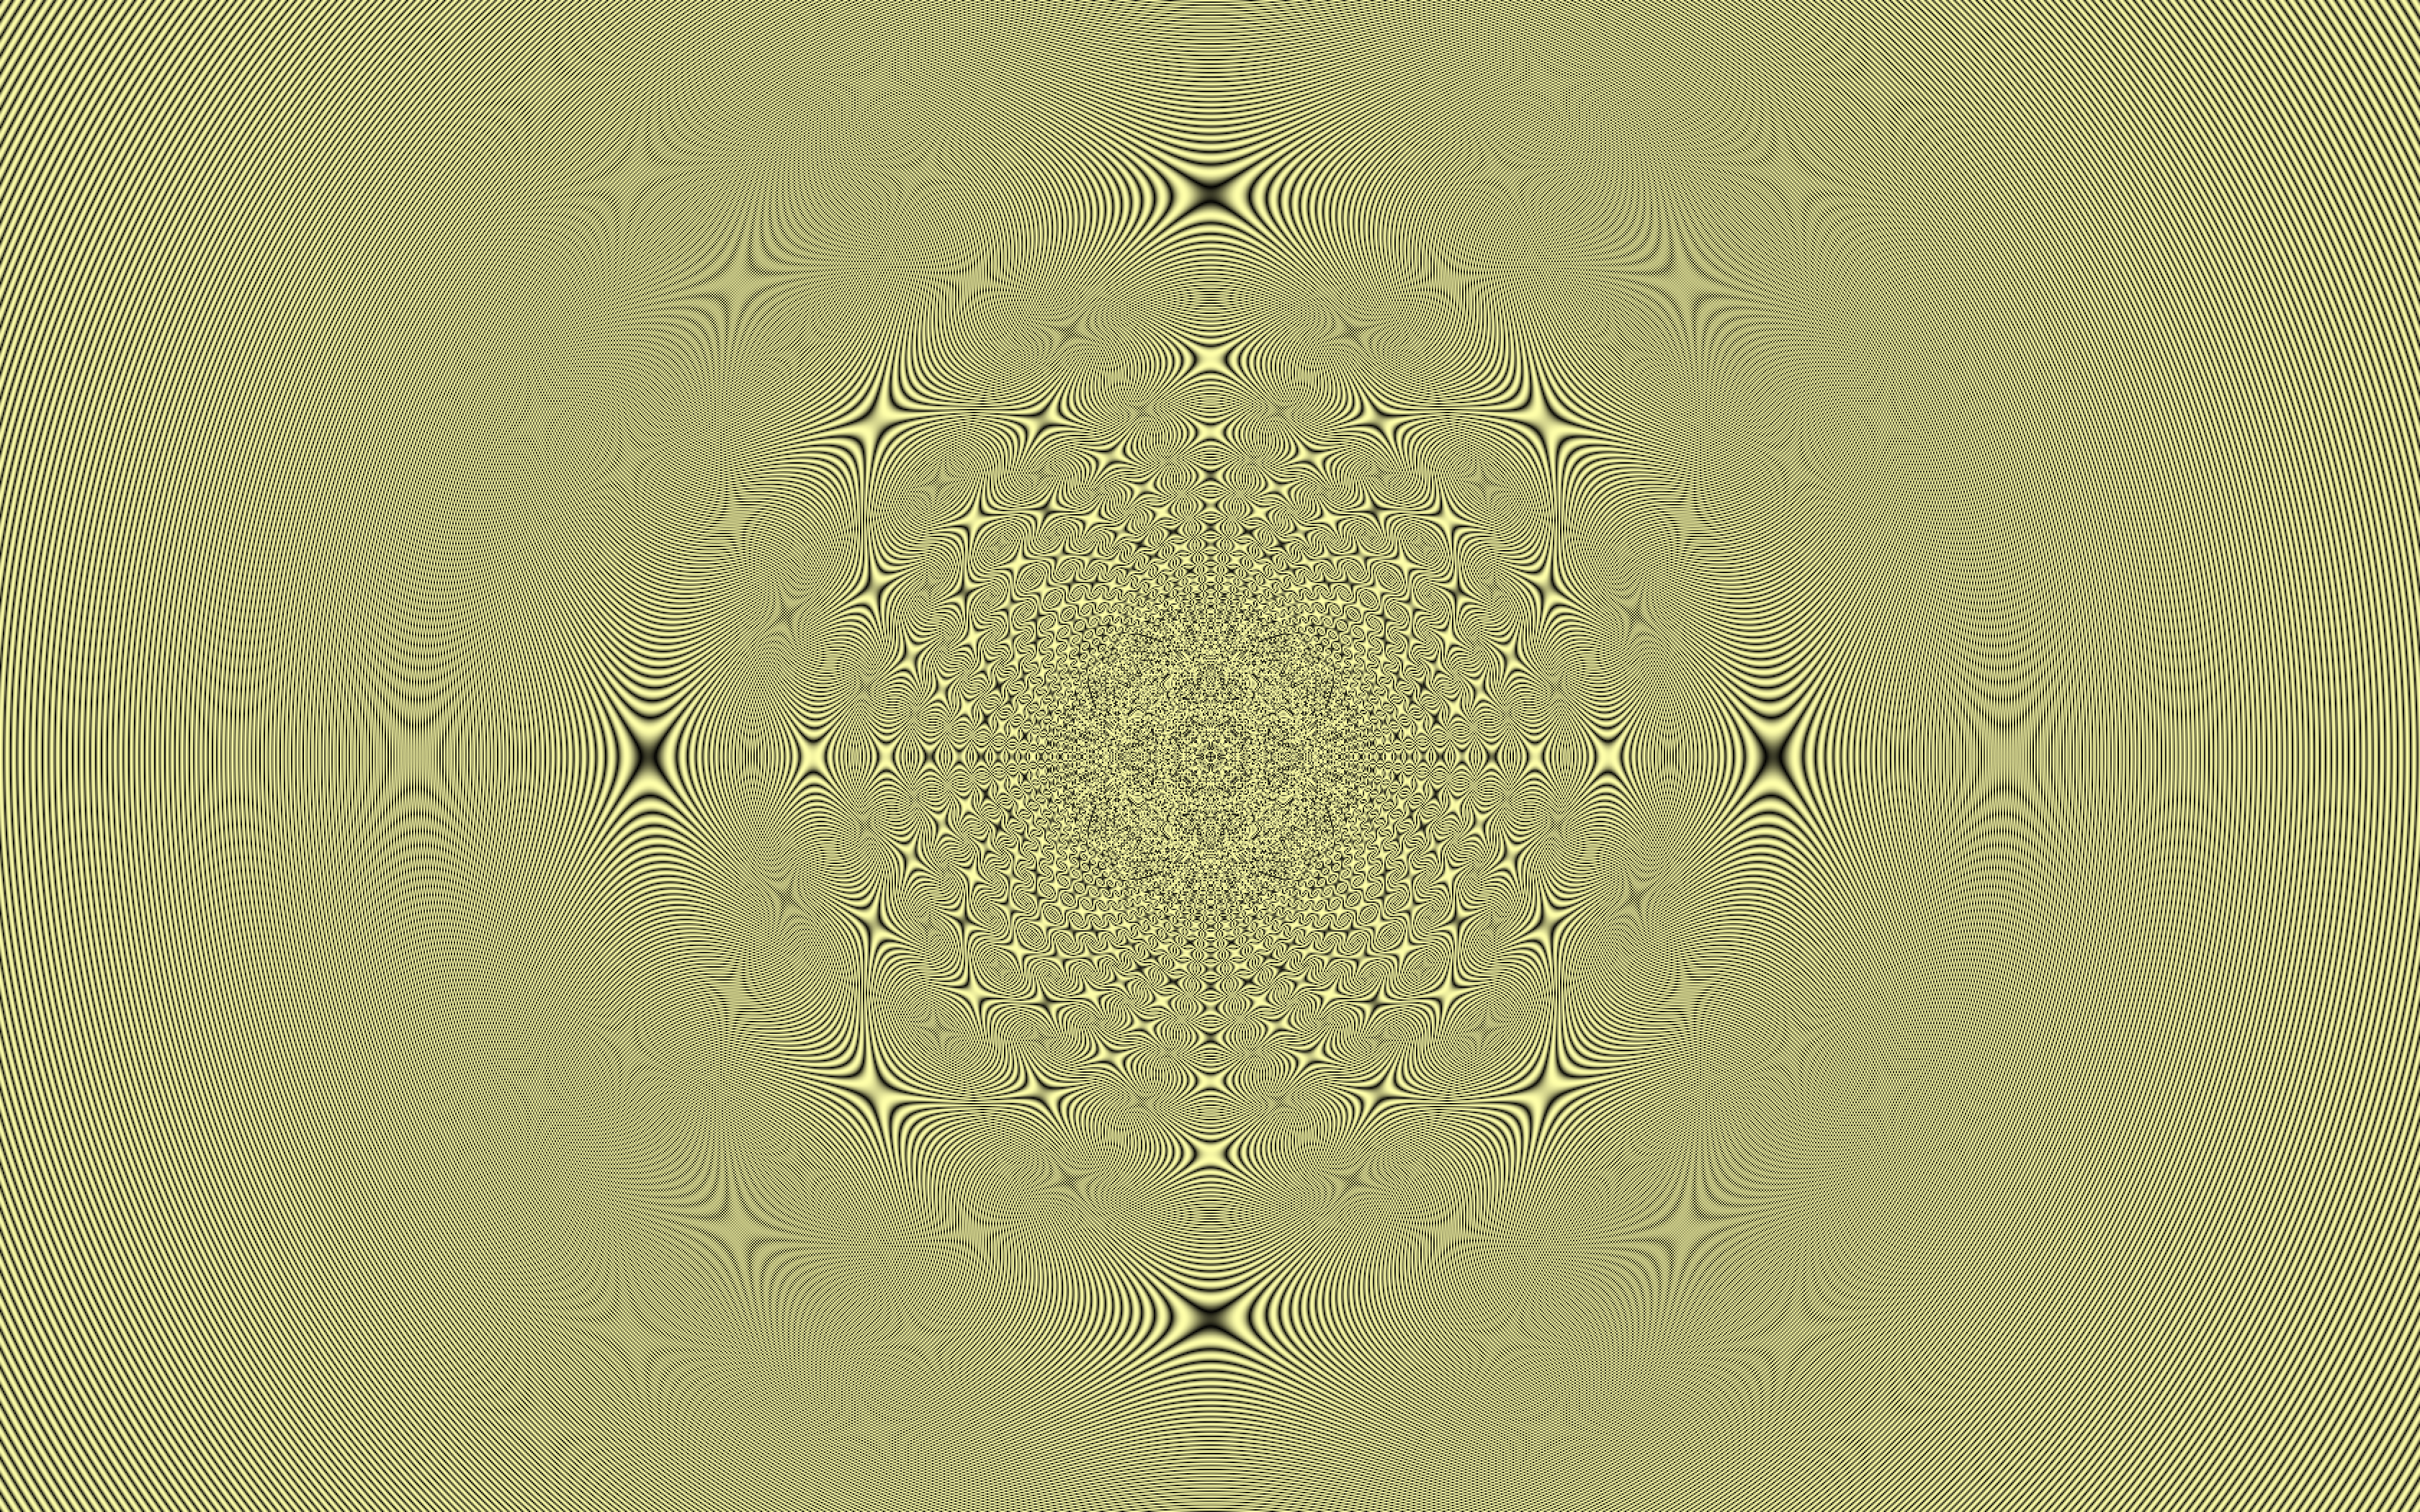
\includegraphics[trim={10cm 0 10cm 0}, clip, width=.7\textwidth]{inverted.png}
\caption{Inverted. Visualization with $\alpha = 1$ and $\lambda = -.5$}
\label{fig:inverted}
\end{figure}
\begin{figure}[h]
\centering
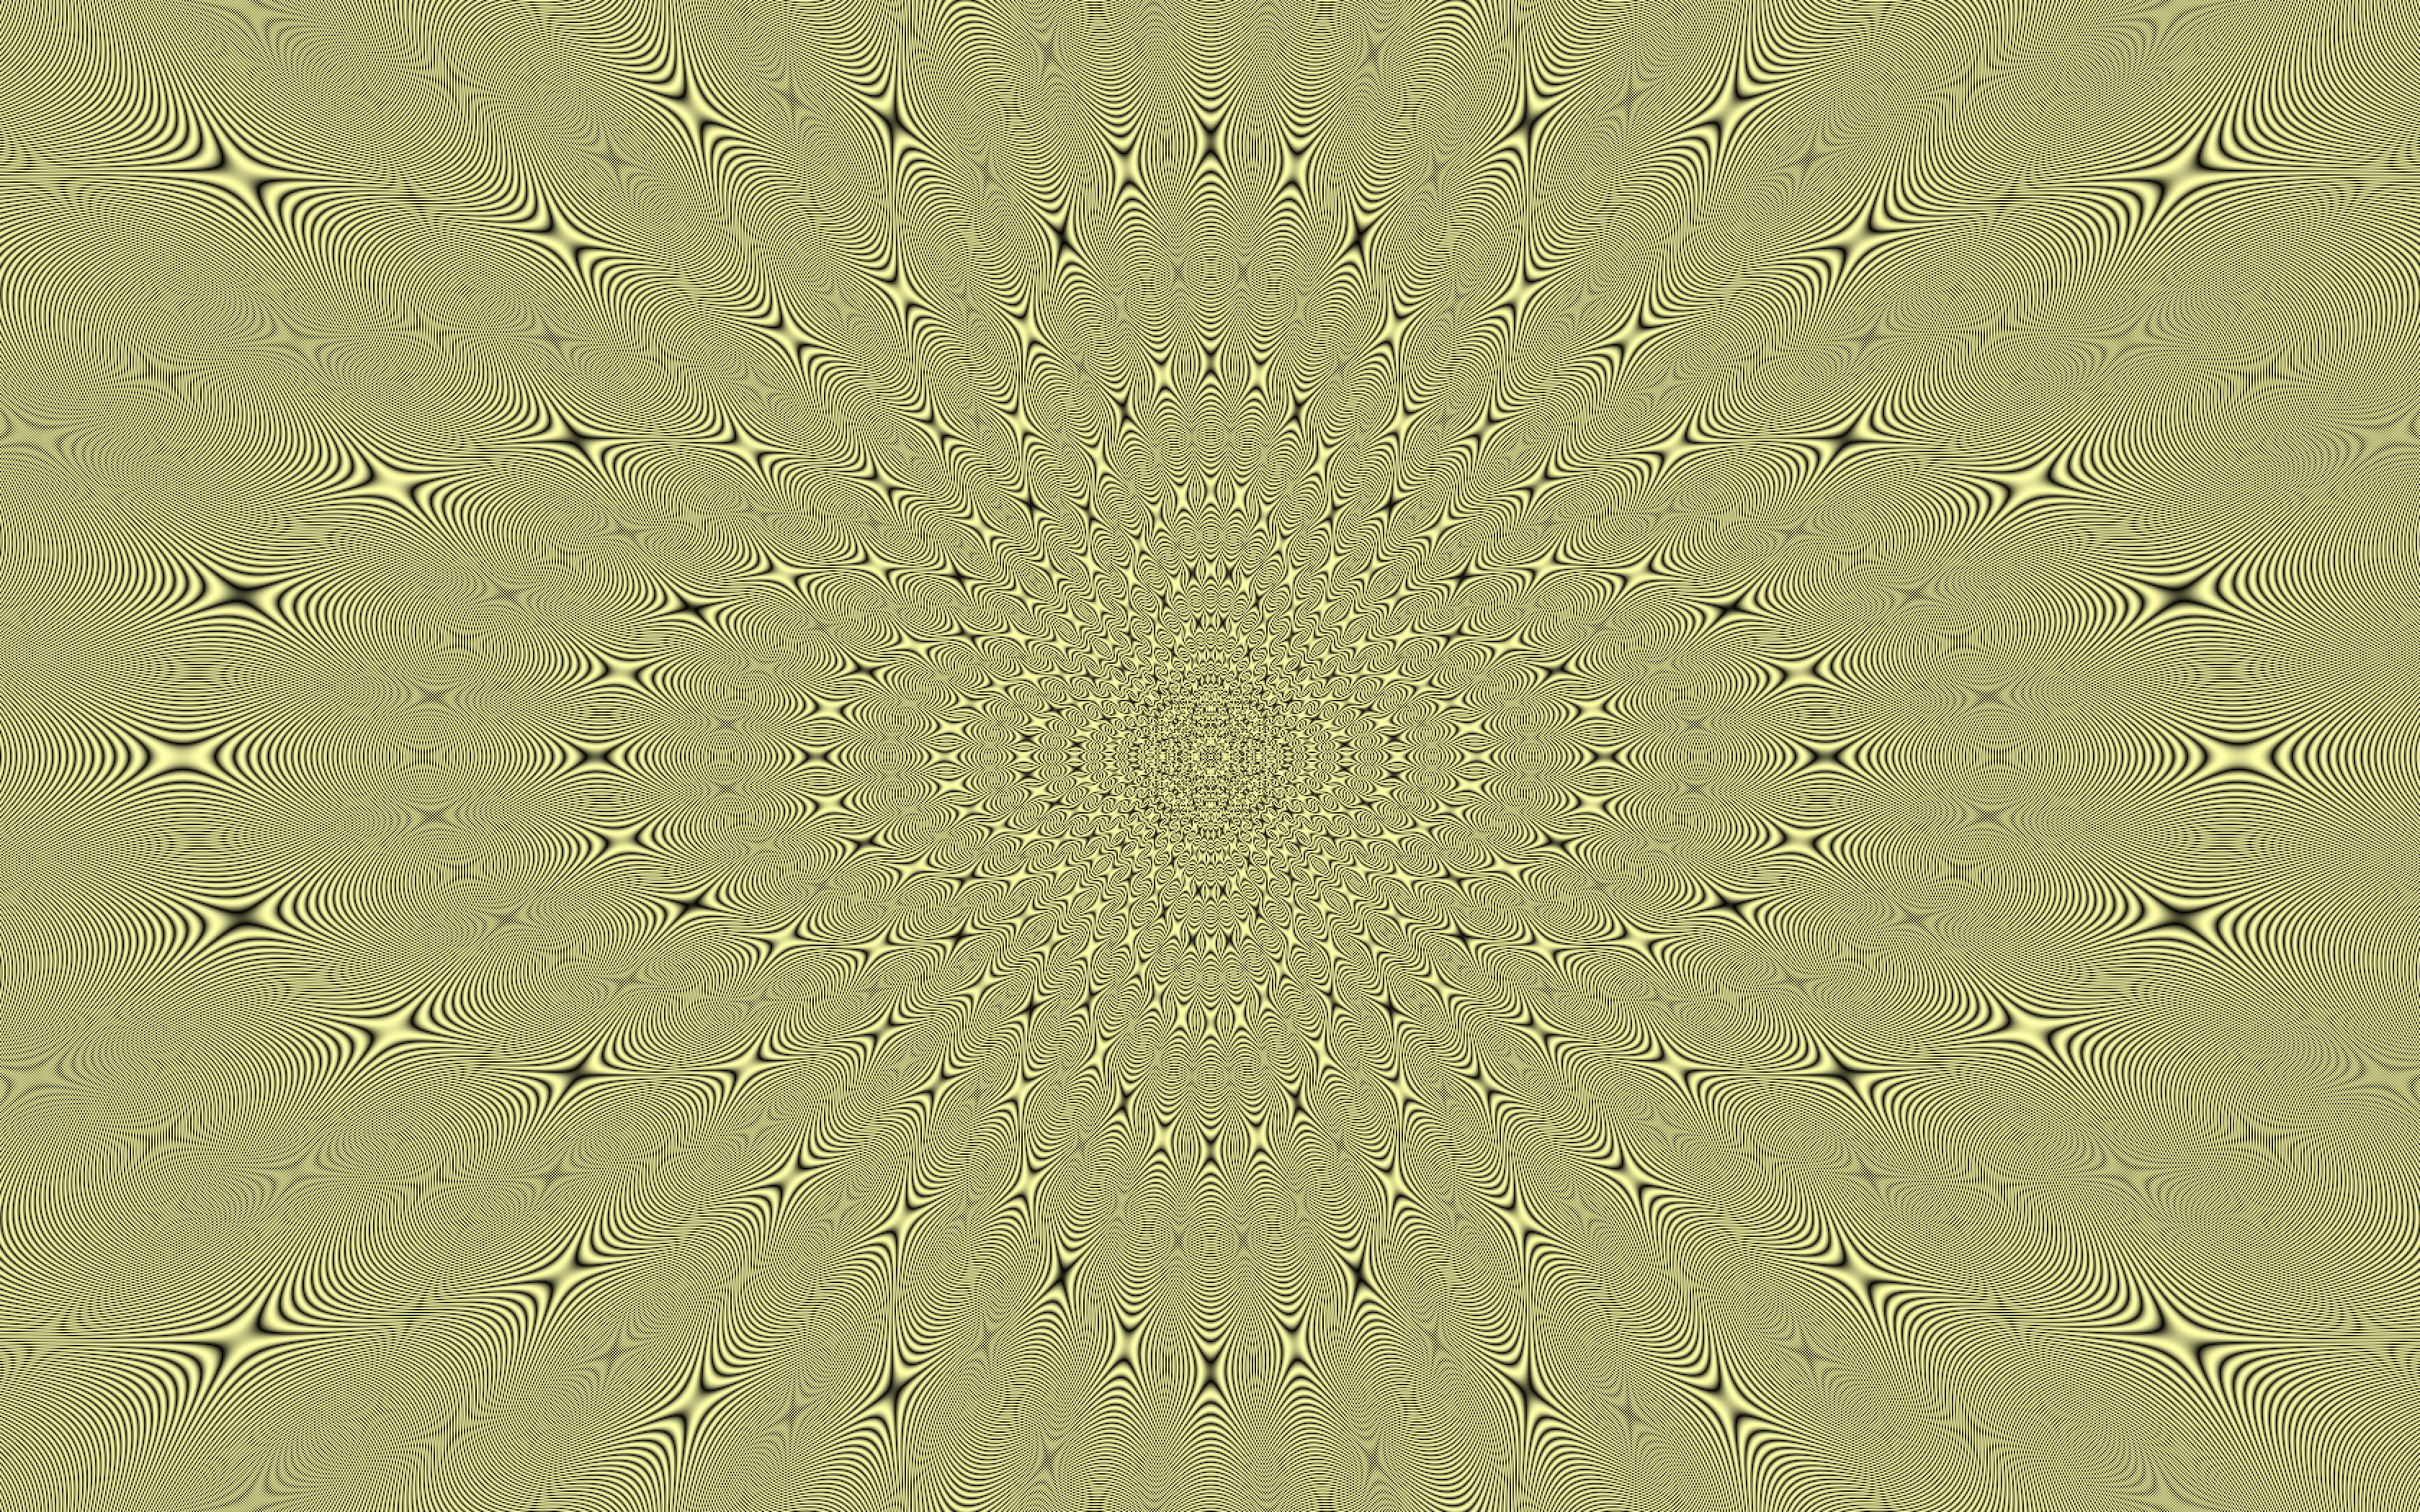
\includegraphics[trim={10cm 0 10cm 0}, clip, width=.7\textwidth]{concave-inverted.png}
\caption{Concave/Inverted. Visualization with $\alpha = 2$ and $\lambda = .35$}
\label{fig:concaveinverted}
\end{figure}
\begin{figure}[h]
\centering
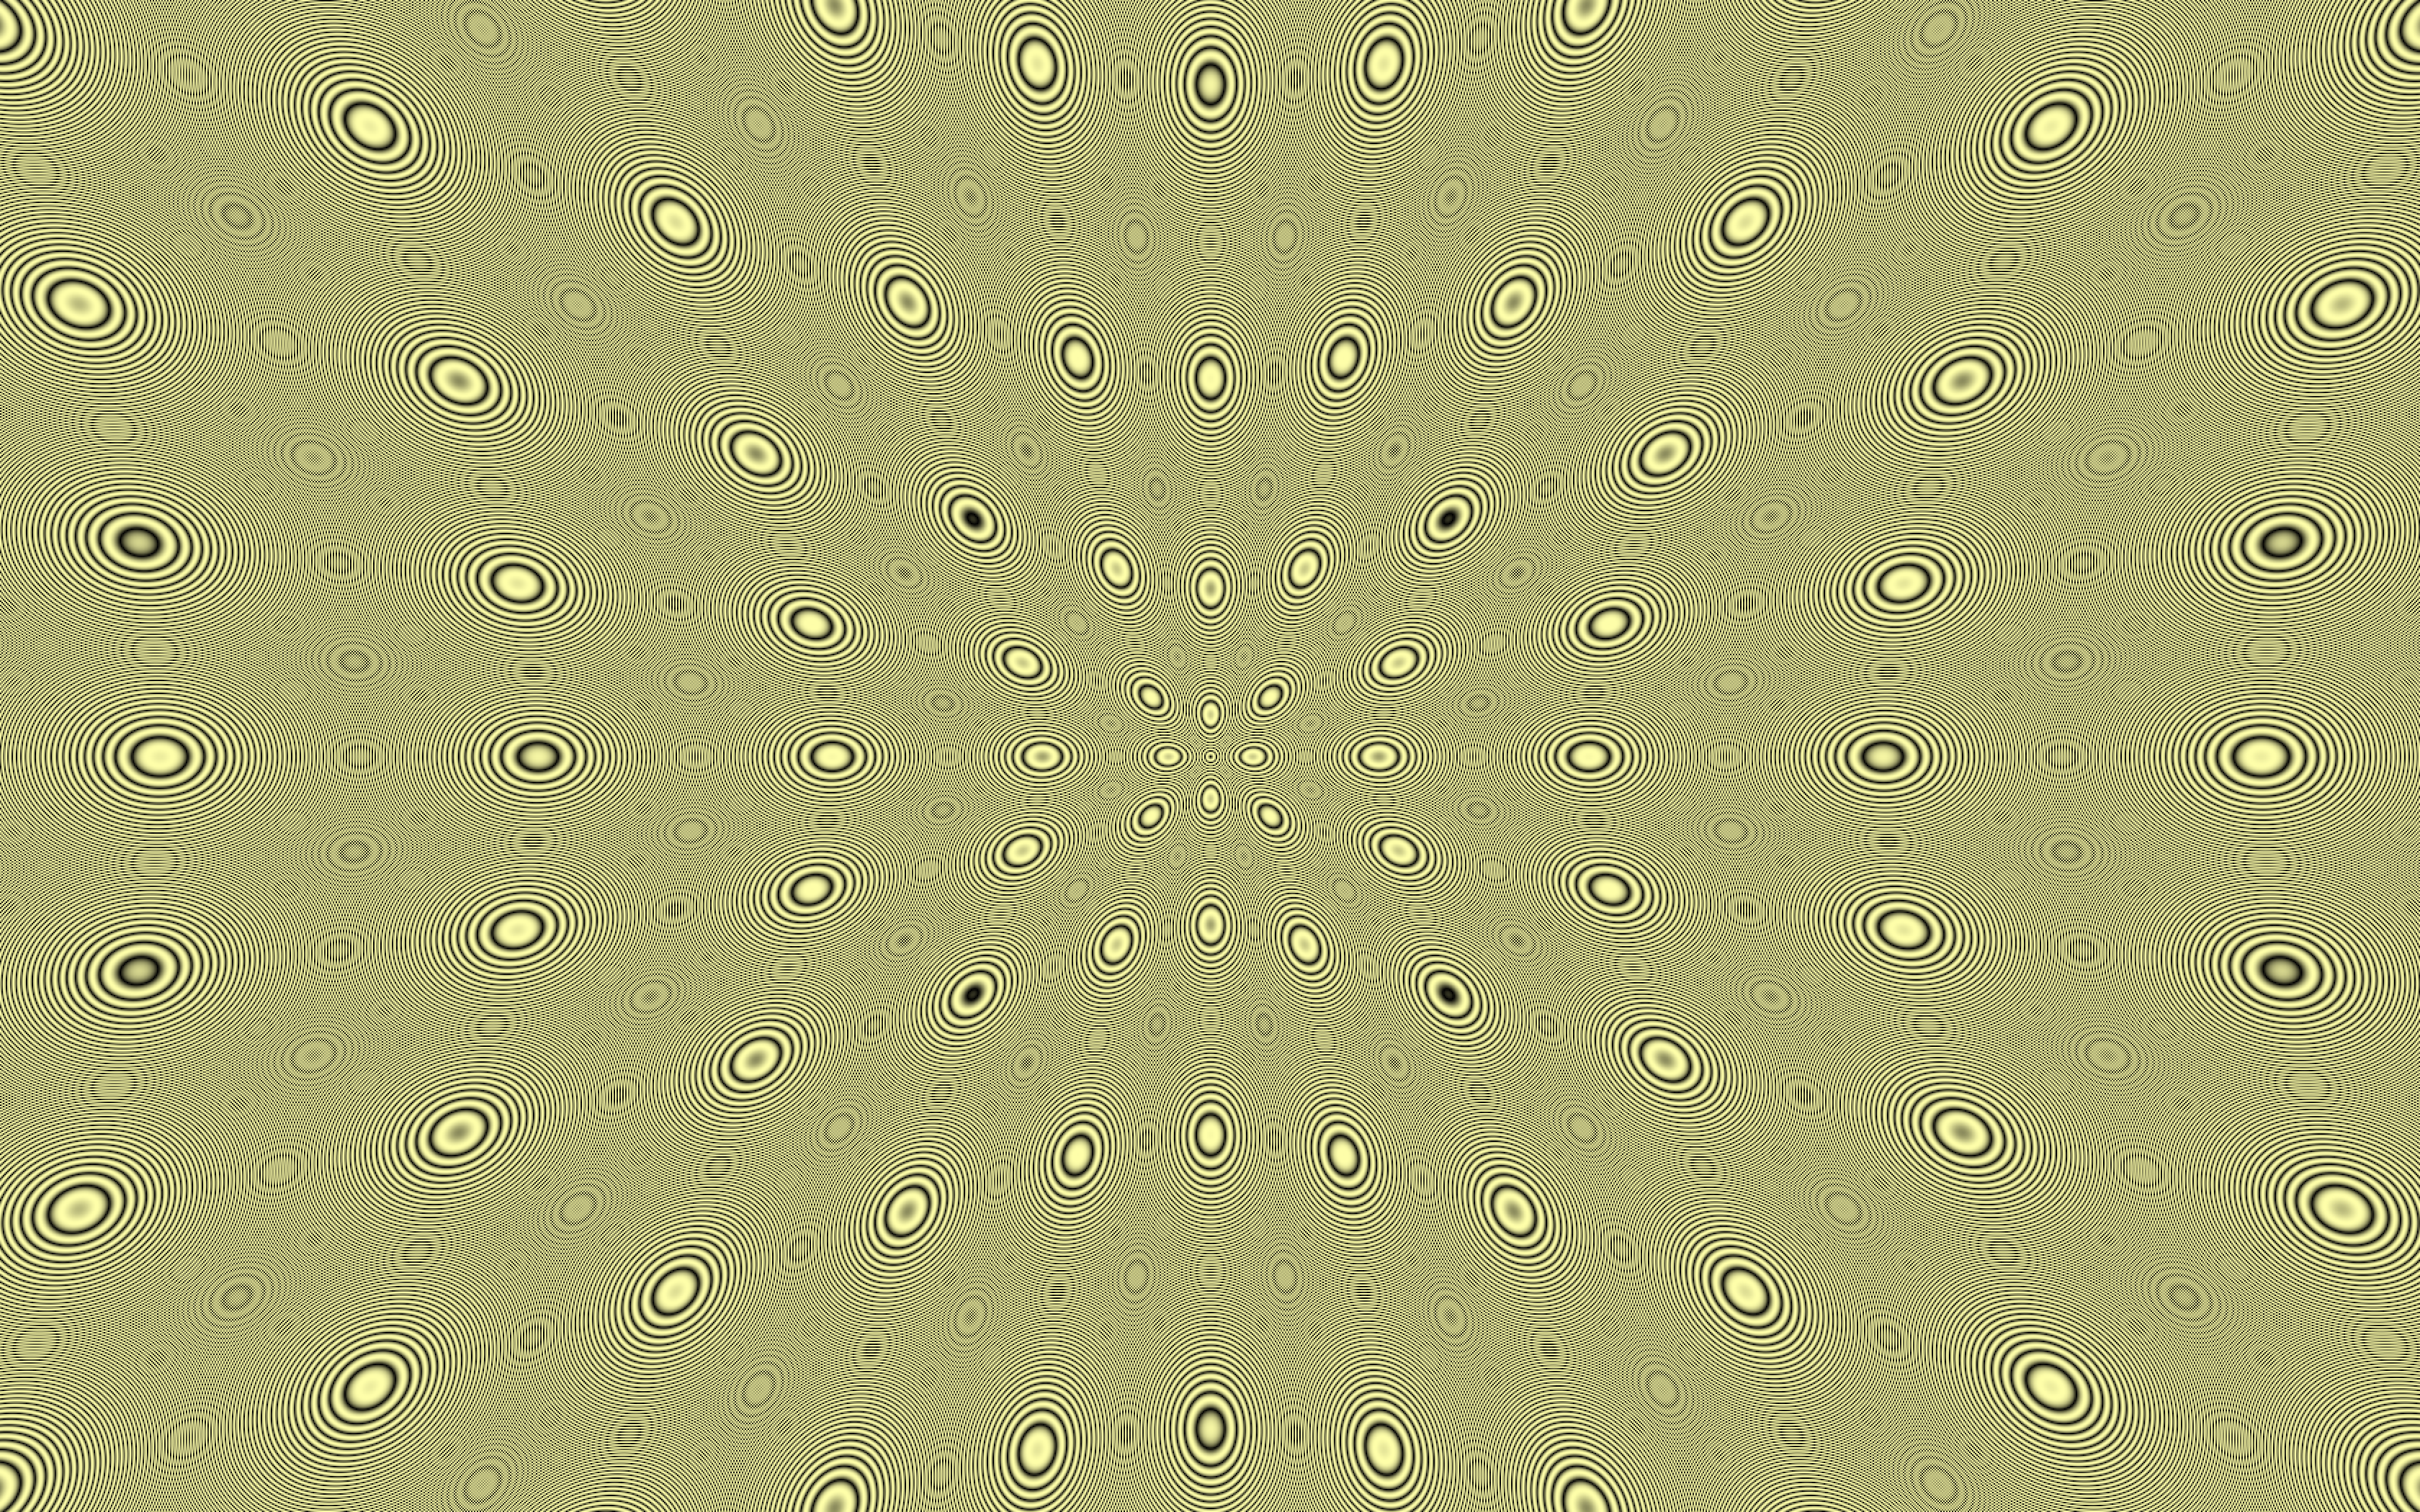
\includegraphics[trim={10cm 0 10cm 0}, clip, width=.7\textwidth]{concave.png}
\caption{Concave. Visualization with $\alpha = 1$ and $\lambda = .75$}
\label{fig:concave}
\end{figure}
\begin{figure}[h]
\centering
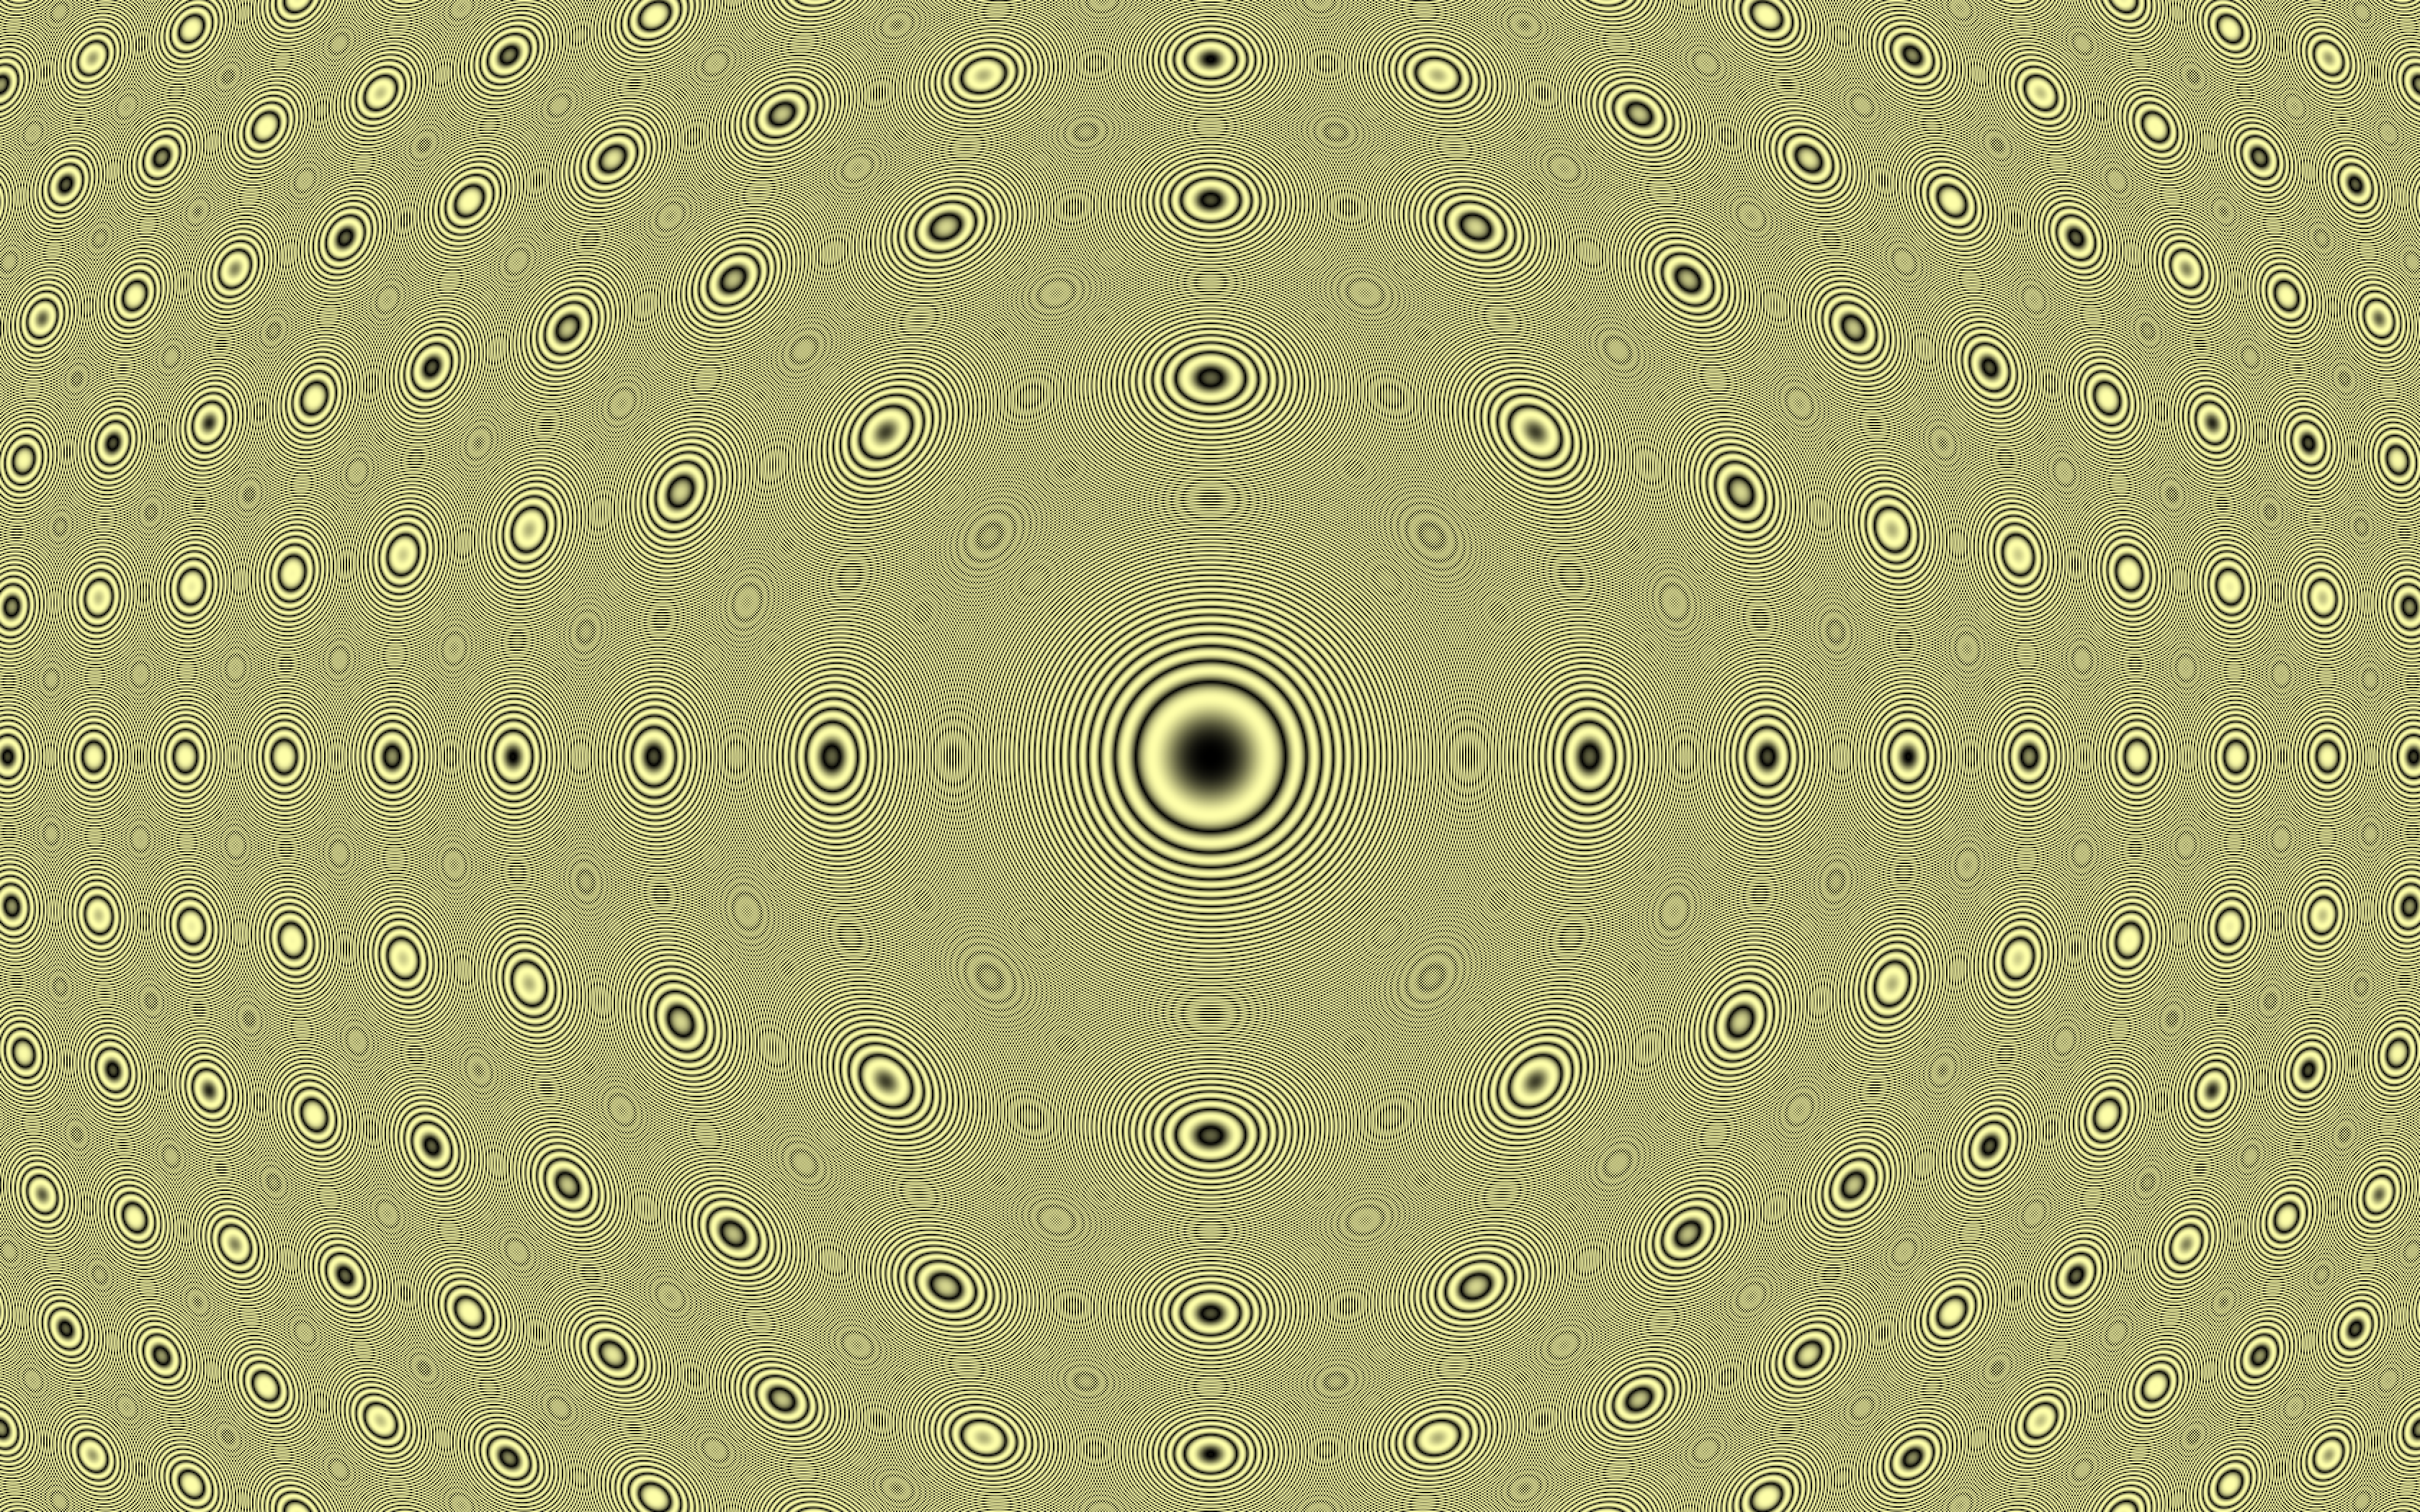
\includegraphics[trim={10cm 0 10cm 0}, clip, width=.7\textwidth]{convex.png}
\caption{Convex. Visualization with $\alpha = 1$ and $\lambda = 1.4$}
\label{fig:convex}
\end{figure}
\end{subsection}
\end{section}
\clearpage
\begin{section}{Mathematical Basis}
How can we produce such a variable pattern from such a simple function? How do we get this recursive nature? The answer lies in modular arithmetic, and the way that the function is displayed on the screen using pixels.\\

\begin{figure}[h]
\centering
\includegraphics[width=.7\textwidth]{plot3d1.png}
\caption{3D-Plot from $(-10, -10)$ to $(10, 10)$. $z$ values are $f(x, y)$}
\label{fig:wolfFar}
\end{figure}
\begin{figure}[h]
\centering
\includegraphics[width=.7\textwidth]{plot3d2.png}
\caption{3D-Plot from $(8 -1)$ to $(10, 1)$. $z$ values are $f(x, y)$}
\label{fig:wolfClose}
\end{figure}

We created a three dimensional plot of what the output should be with $\alpha, \lambda = 1$. \reffig{fig:wolfFar} from $(-10, -10)$ to $(10, 10)$. Then, we have the same graph from $(8, -1)$ to $(10, 1)$ \reffig{fig:wolfClose}. If we look closely at the area, they appear completely different in the two plots. This is due to the sampling of the pixels -- eventually $\alpha (x^2 + y^2)^\lambda$ becomes so large it has a slope greater than 255 for every pixel. At certain frequencies, the slope is great enough for the function to create another parabola. \\

Suppose we take the cross-section $f(x, 0) = x^2\mod 255$ with $\alpha, \lambda = 1$. Obviously, for $x^2 < 255$ forms a parabola. However, when do we form a new parabola? Note that the new values only have to line up for $x\in \mathbb{Z}$
\begin{align*}
(x - k\cdot 255)^2 \mod 255 &\equiv x^2 - 255k\cdot x + (255k)^2 \mod 255\\
&\equiv x^2 \mod 255
\end{align*}

\begin{figure}[h]
\centering
\includegraphics[width=\textwidth]{parabola1.png}
\caption{Cross-Section $f(x, 0)$. Note every integer value of the blue line is equal to the integer value of the orange one. The blue line is $f(x, 0)$, and the orange is the new parabola we see on screen.}
\label{fig:parabola1}
\end{figure}

Note that this works for $k\in \mathbb{N}$ and integer values of $x$ -- otherwise the modulo would not go to zero. However, this implies that every $255k$ pixels we get a new parabola that is exactly the same as the original in the center. This is shown in \reffig{fig:parabola1}. The position of the pixel is represented by the dotted line, the blue line represents our function $f(x, y)$, and the orange line is the parabola that is formed by sampling a position of $f(x, y)$ at every pixel.\\

Notice that we have two `bands' for every pixel -- we call this a 2nd Harmonic. We, in fact, have all integer harmonics (with a high enough $\alpha$), and we even have half harmonics that are between the two. If you look at \reffig{fig:vizlarge} the 0th harmonic is in the center, 1st harmonics to the left and right, and half-harmonics in between. If you zoom up, you will notice that this half harmonic is a combination of the 0th harmonic and the 1st that alternates every pixel.\\

When $\alpha$ is increased, the non-zero harmonics oscillate as multiple bands move through the pixels. This is important for creating an animation for the visualization. We notice that given an $\alpha$, there's a minimum in the parabola at $x = 255 - (\alpha - 1)255$. So, as we're increasing $\alpha$, we reach a new zero minimum zero at $\alpha = k/255 + 1$ when $0 \le k < 255$ for $x = 255 + k$ and $(\alpha -1)255$. This implies that if we change alpha to increase by $1/255$ over one second, the first harmonic will make a complete oscillation in one second. This fact is very useful to us in the music generating process, since it will allow us to make the visualization in tune with the music. 
\end{section}
\begin{section}{Controlling}
Suppose we are increasing $\alpha$ by a constant rate of $1/255$. As we found before, the $n$th harmonic will oscillate completely over $1/n$ seconds. This is useful for matching the tempo and beats of the underlying music. For example, let's suppose our song has a certain $BPM$, the change in alpha over time for the first harmonic would be an ideal 
\[\Delta \alpha = \frac{1/255 BPM}{60}\]

Currently our controller only modifies $\lambda$ to be in the range $.5 \le \lambda \le 1.5$, which makes it bulge inwards or outwards. We modify $\lambda$ based on a floating distribution of the current pitch of a note being played. We have $\alpha$ increase according to the tempo, however, we transition the value of $\alpha$ to a very high, low, or medium value depending on the tempo, placing different tempos in bands with predetermined values of $\alpha$ that we will use. The method for mapping this is discussed in our general project file. 
\end{section}
\end{document}

% boring, normal, etc images
% wolfram close, far on 3d plot

%boring alpha .1
%linear large 10
%linear small .001
%convex, concave 1 .75, 1.4
%inverted -.5
%inverted/concave 2, .35